\chapter{相關應用}

\section{電子鼻}
\subsection{人類嗅覺的限制}
即使在現代科技中,依然有許多行業需要依靠人體的嗅覺作為判斷依據。曾經有人做過
一個紅酒實驗 \cite{hodgson_2008} ,他觀察了許多種紅酒,發現同一種紅酒在兩次
紅酒競賽獲得的成績,其相關性不高。此外,人體的感官也可能因為年齡或者其他變因
而產生誤差 \cite{Hugh2015} 。因此,依靠人類的感官作為判斷依據的可靠度值得懷疑。
\subsection{原理}
電子鼻是一種用來模擬鼻子功能的電子儀器。利用多個感測器組合而成的一個整體,
而氣體在接觸到電子鼻時,內部的每個感測器會產生不同程度的電阻變化,因此透過
比對不同變化,即可產生電子指紋圖(electronic fingerprint)並辨識出
此為何種氣體,更甚者可計算出該氣體濃度。 \footnote{\url{https://scitechvista.nat.gov.tw/Article/C000003/detail?ID=e1893f7f-9eda-4ed7-ada0-dc226bfc1d57}}
\subsection{應用}
隨著科技演進,越來越多技術可以應用在電子鼻上。舉例來說,人工智慧可以運用
在電子鼻上,幫助提昇效能,使電子鼻能夠被運用在更複雜的環境,例如檢測膀胱癌。 \footnote{\url{https://case.ntu.edu.tw/blog/?p=36043}}
\begin{figure}[H]
	\centering
	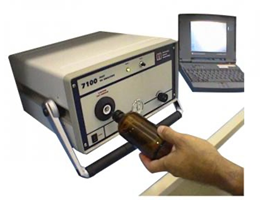
\includegraphics[width=0.5\textwidth]{pic/nose.png}
\end{figure}

\section{人體氣味感測實例-三點比較式嗅袋法}
利用多個人嗅聞的結果下去取平均值,減少誤差的人工測試法(三點比較式嗅袋法\footnote{\url{https://www.epa.gov.tw/DisplayFile.aspx?FileID=96A2ABC05E2DB1F6}})
- 人體嗅覺是否能察覺有害氣體。
\subsection{作法}
\begin{enumerate}
	\item 先將某個待採樣氣體放於三個袋子其中一袋。並請多個測試員聞袋子。
	\item 該測試會不斷嘗試稀釋袋內空氣,當多數測試員能夠聞出味道的最低濃度,再去推算稀釋了幾倍,
		即可得到原始氣體濃度。
\end{enumerate}

\section{氣味感測器實例應用}
	\subsection{油管漏油事件}
	一旦漏油情況發生,即會對附近水域造成大範圍影響。因此,在水域附近裝有電子鼻,即可在漏油情況發生
	第一時間發現,並且以較快速度解決危機,減少損害面積。 \footnote{\url{https://www.tiri.narl.org.tw/Files/Doc/Publication/InstTdy/145/01450060.pdf}}